\documentclass[%
%draft,%
11pt,%
%oneside,%
twoside,%‡
%twocolumn,%
titlepage,%
%fleqn,%
%a4page,%
german,%
headsepline%
]{scrartcl}

\usepackage{lastpage}
\usepackage{geometry}
\usepackage{graphicx}
\usepackage[utf8]{inputenc}
\usepackage[ngerman]{babel}
\usepackage{lscape}
\usepackage[framemethod=TikZ]{mdframed}
\usepackage[most]{tcolorbox}
\usepackage{mymath}
\usepackage{units}
\usepackage{nicefrac}
\usepackage{pgf,tikz}
\usetikzlibrary{arrows}
\usepackage{colortbl}
\usepackage{hhline}
\usepackage{multirow}
\usepackage[extendedchars]{grffile}
\usepackage{caption}
\usepackage{multicol,calc}
\usepackage{blindtext}
\usepackage{pdfpages}
\usepackage{hyperref}
\usepackage{framed}
\usetikzlibrary{arrows}
\usetikzlibrary{positioning}
\usetikzlibrary{shadows}
\usepackage{pgfplots}
\pgfplotsset{compat=1.15}
\usepackage{mathrsfs}

\usepackage{ocg}
\usepackage{fontawesome}
\usepackage{xcolor}

\usepackage{marginnote}
\usepackage
%[draft]%
{qrcode}
\qrset{height=9ex}

\usepackage{longtable}
\usepackage{listings}
\usepackage{wrapfig}

\usepackage{fontawesome} % Oder FontAwesome, falls du ein Augensymbol aus einer
\definecolor{lightgray}{rgb}{0.7, 0.7, 0.7}
\newcommand{\faEyeLightGray}{\textcolor{lightgray}{\faEye}} % Custom command for the gray eye icon

\newcommand{\geogebralink}{\href{https://www.geogebra.org/calculator}{\texttt{geogebra.org}}}

% Command, um Tabellen-Spalten anzupassen
\newcommand{\spaltenheight}{\rule{0mm}{3ex}}
\newcommand{\spaltenwidth}{\rule{3cm}{0mm}}
\newcommand{\spaltensep}{\\[1ex]}
\doublerulesepcolor{white}
\definecolor{lightyellow}{rgb}{1,1,0.8}
\definecolor{Gray}{gray}{0.9}

\pagestyle{headings} % gemachte Einstellungen anwenden

% Farbig umrahmte Umgebung Satz
\definecolor{myblizzardblue}{HTML}{87CEEB}

\newcounter{satzz}[section]\setcounter{satzz}{0}
\renewcommand{\thesatz}{\arabic{section}.\arabic{satzz}}

\newenvironment{csatz}[1][]{%
    \refstepcounter{satzz}
 
    \ifstrempty{#1}%
    % if condition (without title)
    {\mdfsetup{%
        frametitle={%
            \tikz[baseline=(current bounding box.east),outer sep=0pt]
            \node[anchor=east,rectangle,fill=myblizzardblue]
            {\strut Satz~\thesatz};}
        }%
    % else condition (with title)
    }{\mdfsetup{%
        frametitle={%
            \tikz[baseline=(current bounding box.east),outer sep=0pt]
            \node[anchor=east,rectangle,fill=myblizzardblue]
            {\strut Satz~\thesatz:~#1};}%
        }%
    }%
% for both conditions
    \mdfsetup{%
        innertopmargin=10pt,linecolor=myblizzardblue,%
        backgroundcolor=whitesmoke,%
        linewidth=2pt,topline=true,%
        frametitleaboveskip=\dimexpr-\ht\strutbox\relax%
    }
 
\begin{mdframed}[]\relax}{%
\end{mdframed}}

% Farbig umrahmte Umgebung Theorem
 
\definecolor{mygraphblue}{HTML}{84B7E1}
\definecolor{whitesmoke}{HTML}{F5F5F5}

\newcounter{theo}[section]\setcounter{theo}{0}
\renewcommand{\thetheo}{\arabic{section}.\arabic{theo}}

\newenvironment{ctheo}[2][]{%
    \refstepcounter{theo}
 
    \ifstrempty{#1}%
    % if condition (without title)
    {\mdfsetup{%
        frametitle={%
            \tikz[baseline=(current bounding box.east),outer sep=0pt]
            \node[anchor=east,rectangle,fill=mygraphblue]
            {\strut Theorem~\thetheo};}
        }%
    % else condition (with title)
    }{\mdfsetup{%
        frametitle={%
            \tikz[baseline=(current bounding box.east),outer sep=0pt]
            \node[anchor=east,rectangle,fill=mygraphblue]
            {\strut Theorem~\thetheo:~#1};}%
        }%
    }%
% for both conditions
    \mdfsetup{%
        innertopmargin=10pt,linecolor=mygraphblue,%
        backgroundcolor=whitesmoke,%
        linewidth=2pt,topline=true,%
        frametitleaboveskip=\dimexpr-\ht\strutbox\relax%
    }
 
\begin{mdframed}[]\relax}{%
\end{mdframed}}

% Farbig umrahmte Umgebung Definition
 
 \definecolor{emerald}{HTML}{50C878}

\newcounter{deff}[section]\setcounter{deff}{0}
\renewcommand{\thedeff}{\arabic{section}.\arabic{deff}}

\newenvironment{cdef}[1][]{%
    \refstepcounter{deff}
 
    \ifstrempty{#1}%
    % if condition (without title)
    {\mdfsetup{%
        frametitle={%
            \tikz[baseline=(current bounding box.east),outer sep=0pt]
            \node[anchor=east,rectangle,fill=emerald]
            {\strut Definition~\thedeff};}
        }%
    % else condition (with title)
    }{\mdfsetup{%
        frametitle={%
            \tikz[baseline=(current bounding box.east),outer sep=0pt]
            \node[anchor=east,rectangle,fill=emerald]
            {\strut Definition~\thedeff:~#1};}%
        }%
    }%
% for both conditions
    \mdfsetup{%
        innertopmargin=10pt,linecolor=emerald,%
        backgroundcolor=whitesmoke,%
        linewidth=2pt,topline=true,%
        frametitleaboveskip=\dimexpr-\ht\strutbox\relax%
    }
 
\begin{mdframed}[]\relax}{%
\end{mdframed}}

% Farbig umrahmte Umgebung Achtung
 
 \definecolor{mygraphred}{HTML}{E26A6A}

\newcounter{merkee}[section]\setcounter{merkee}{0}
\renewcommand{\themerkee}{\arabic{section}.\arabic{merkee}}

\newenvironment{cachtung}[2][]{%
    \refstepcounter{merkee}
 
    \ifstrempty{#1}%
    % if condition (without title)
    {\mdfsetup{%
        frametitle={%
            \tikz[baseline=(current bounding box.east),outer sep=0pt]
            \node[anchor=east,rectangle,fill=mygraphred]
            {\strut Achtung};}
        }%
    % else condition (with title)
    }{\mdfsetup{%
        frametitle={%
            \tikz[baseline=(current bounding box.east),outer sep=0pt]
            \node[anchor=east,rectangle,fill=mygraphred]
            {\strut Achtung:~#1};}%
        }%
    }%
% for both conditions
    \mdfsetup{%
        innertopmargin=10pt,linecolor=mygraphred,%
        backgroundcolor=whitesmoke,%
        linewidth=2pt,topline=true,%
        frametitleaboveskip=\dimexpr-\ht\strutbox\relax%
    }
\begin{mdframed}[]\relax}{%
\end{mdframed}}

%\newtheorem{uebthm}{Übung}[section]
% Umgebung lsg mit dynamischer Referenzierung und Label
\newcommand{\concatueb}[1]{ueb:#1}% Definition für concatueb
\newcommand{\concatlsg}[1]{lsg:#1}% Definition für concatlsg

\newcounter{uebcounter}[section]
\renewcommand{\theuebcounter}{\thesection.\arabic{uebcounter}}  % Zählerformat: Abschnitt.Übung

% Definition einer Übungsumgebung mit dynamischen Labels
\newcommand{\uebh}[2]{%
 \refstepcounter{uebcounter} % Zählt den Übungscounter hoch
 \par\noindent\textbf{Übung \theuebcounter:}\label{\concatueb{#1}} % Label im Format "ueb:1"
    #2
    \hfill\hyperref[\concatlsg{#1}]{\faEyeLightGray}
    \vspace{\parskip}
}

\newenvironment{lsg}[1]{%
    \par\noindent\textbf{Notizen zu Übung \ref{\concatueb{#1}}.}%
    \label{\concatlsg{#1}}
}{%
    \par%
}

\newenvironment{uebenv}[1]{%
    \refstepcounter{uebcounter}
    \par\noindent\textbf{Übung \theuebcounter.}%
    \label{\concatueb{#1}}\hfill\hyperref[\concatlsg{#1}]{\faEyeLightGray}\par
}{%
    \par
}

\newcommand{\definition}[1]{\colorbox{emerald}{#1}}

\setlength{\parindent}{0pt}

\subject{\includegraphics[width=0.618\textwidth]{pictures/springbrunnen.jpg}}
\title{Funktionentypen}
\subtitle{beyond linear}
\author{}
\date{}
\lowertitleback{
\includegraphics[height=1cm]{pictures/gymfmslerbermattlogo.eps}
\hfill%\copyright%
{\begin{tikzpicture}
  % Draw the rounded rectangle and clip the image to it
  \clip [rounded corners=5mm] (0,0) rectangle (1,1); % Adjust dimensions as needed
  \node at (0.5,0.5) {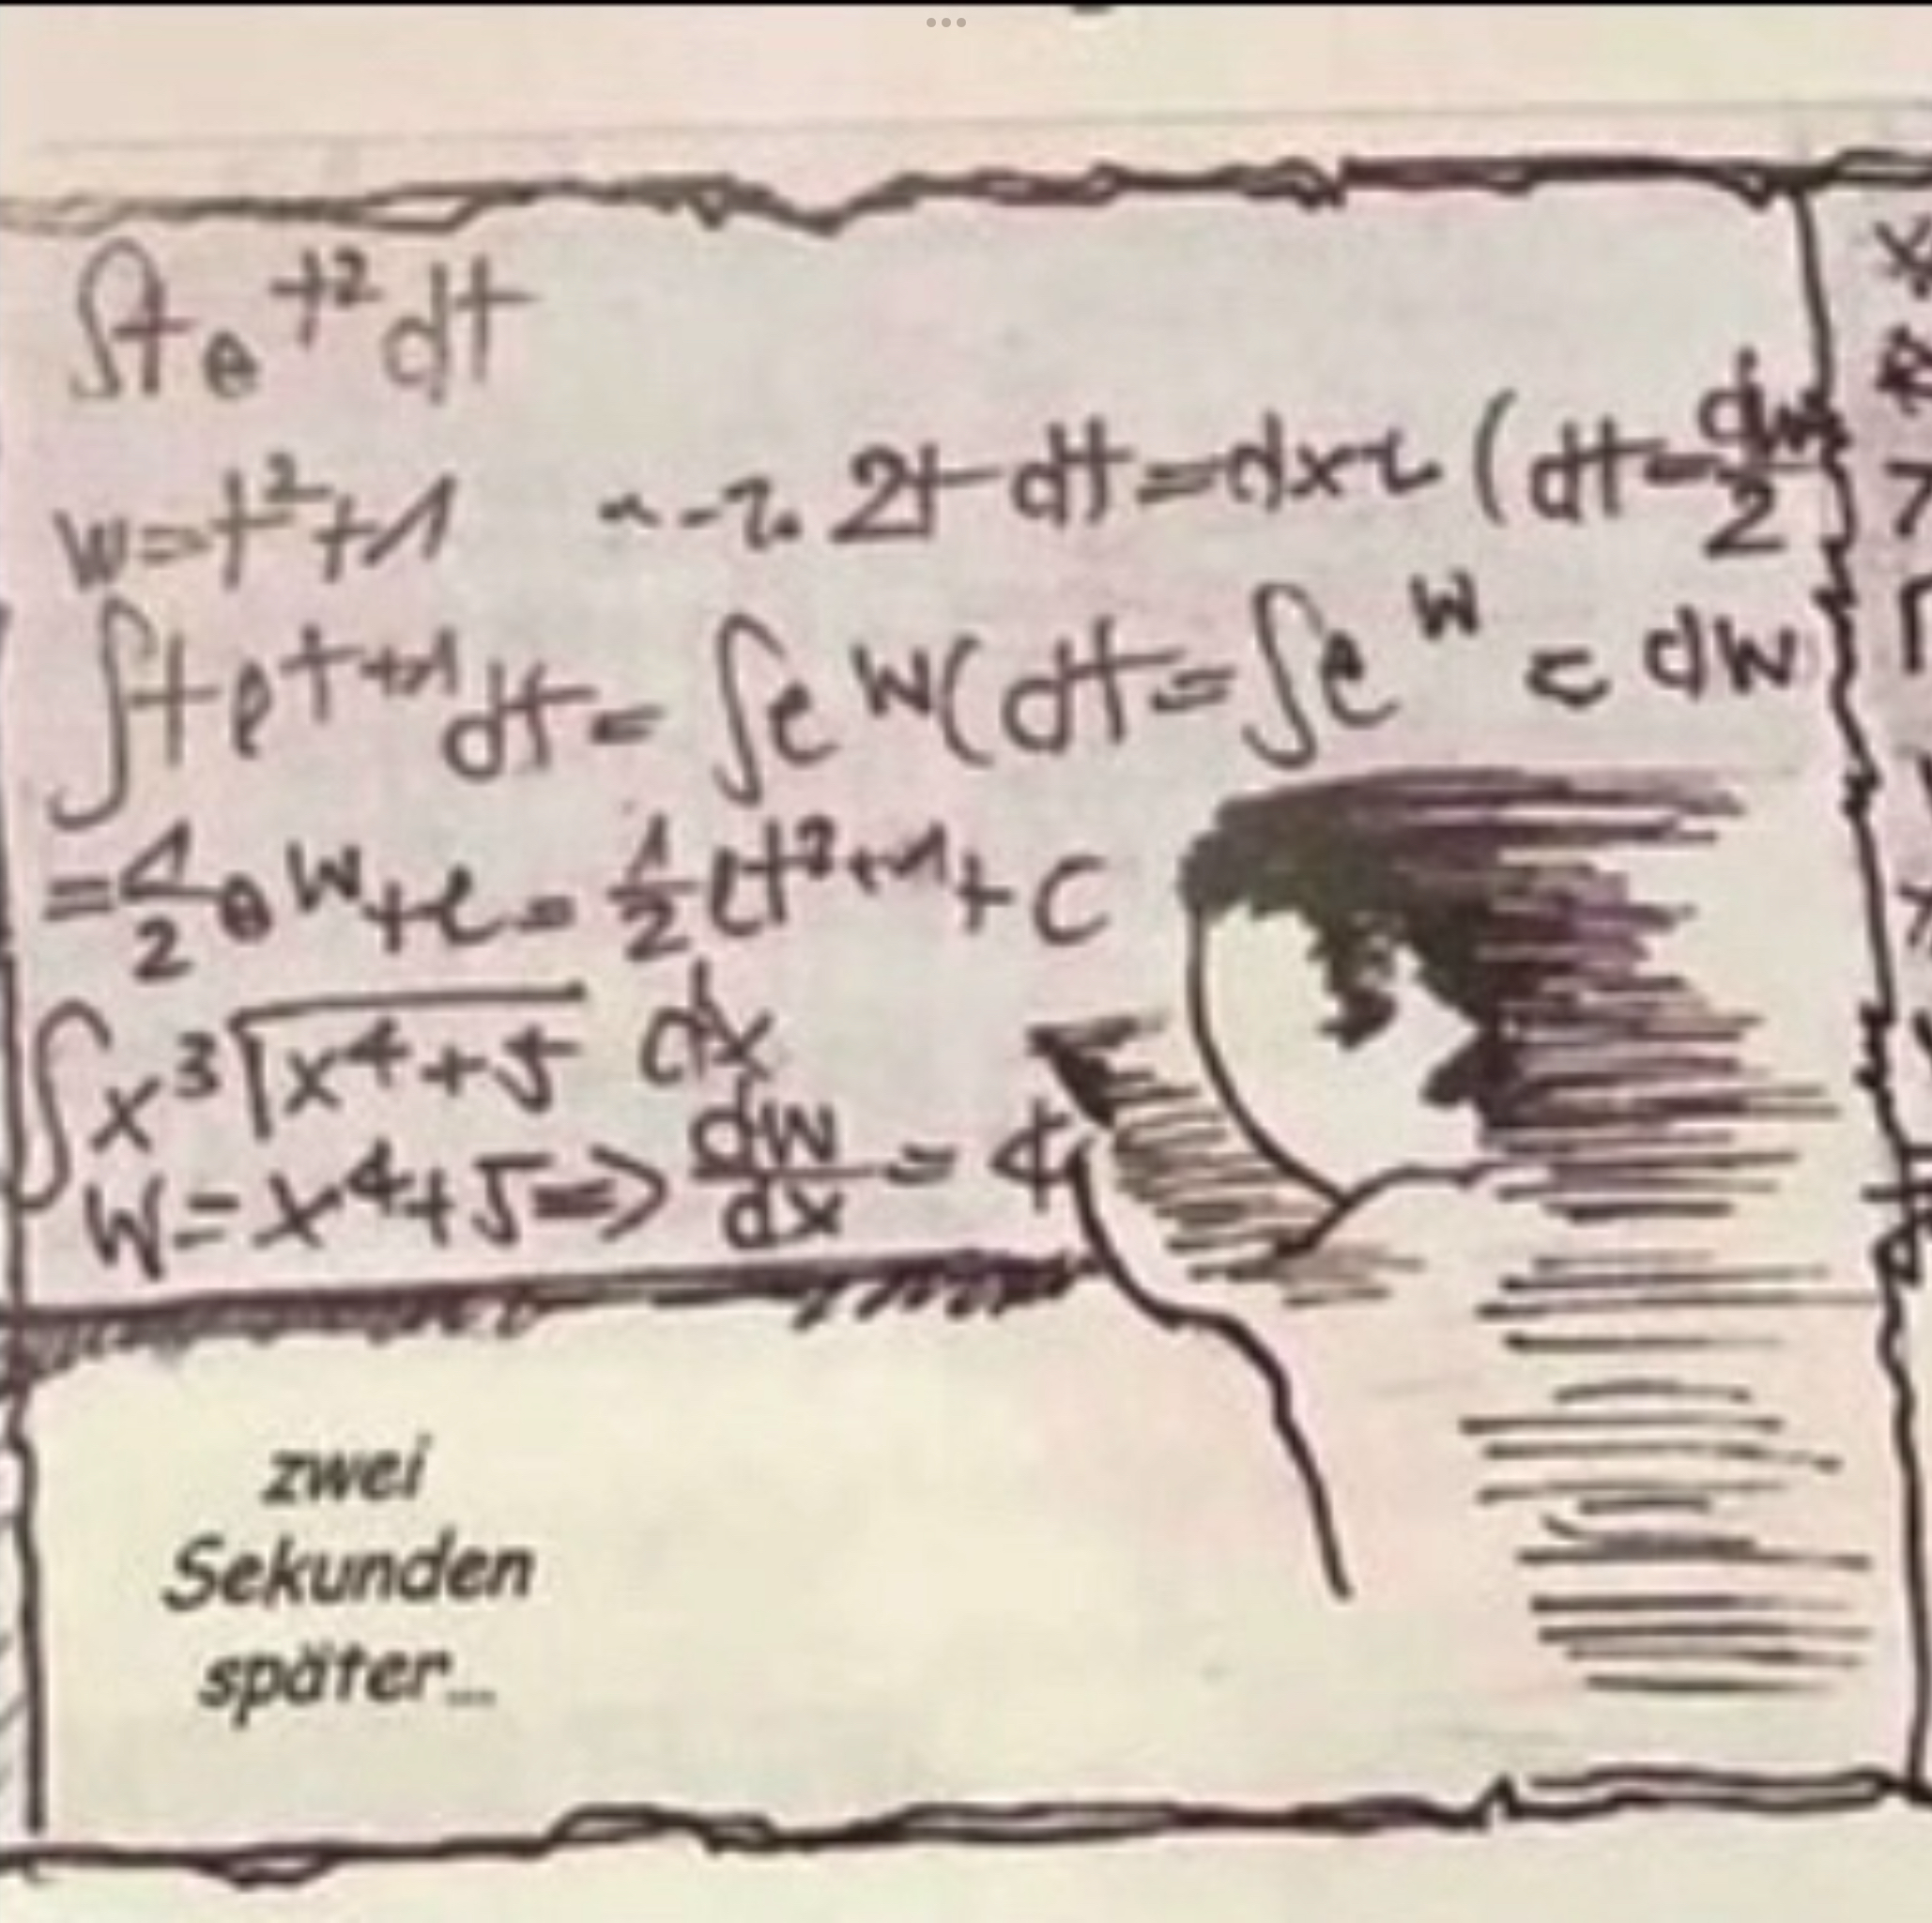
\includegraphics[width=1cm]{pictures/teacher_me_caricatur.png}}; % Adjust width and center image
\end{tikzpicture}}
}


\begin{document}
\maketitle
\tableofcontents
\cleardoublepage

\clearpage
 
\section{Potenzfunktionen}
  
\subsection{Potenzen mit rationalen Exponenten}
\subsubsection{Rückblick}
  \begin{wrapfigure}{r}{0.382\textwidth}
  \begin{center}
    \includegraphics[width=0.382\textwidth]{pictures/title}
  \end{center}
\end{wrapfigure}
Wir wollen unsere Rechenregeln für Potenzen erweitern, um Potenzgesetze
für reelle Zahlen vollumfänglich verstehen und interpretieren zu können.
Wir brauchen dazu folgende, bereits bekannte, Regeln und Begriffe.
\begin{erin}
  Sie
\marginnote{
\qrcode{
https://www.youtube.com/watch?v=du2h6QDXNoo}
}
  kennen die Potenzgesetze. In Kurzform lauten sie:
\begin{align}
  a^n\cdot a^m&=a^{n+m}\\
  a^n\cdot b^n&=(ab)^n\\
  \left(a^n\right)^m&=a^{n\cdot m}\\
  a^{-n}&=\frac{1}{a^n}\\
  a^0&=1
\end{align}

Bisher waren die Exponenten $m$ und $n$ jeweils natürliche Zahlen (oder ausnahmsweise ganze Zahlen). Im
nächsten Abschnitt werden Sie sehen, dass auch rationale Zahlen im Exponenten sinnvoll sind.

Weiter ruft man sich die Definition der $n$-ten Wurzel einer Zahl
in Erinnerung: Die \emph{$n$-te Wurzel} aus einer positiven Zahl
$a$, ist diejenige positive Zahl $b$, deren $n$-te Potenz $a$ beträgt.
Man schreibt dafür $b=:\sqrt[n]{a}$.
\end{erin}

Die Potenzgesetze funktionieren bis anhin tadellos, wenn $m$ und
$n$ ganze Zahlen sind. Was ist, wenn man nun im Exponenten rationale
Zahlen zulässt? Ist $3^{\frac{1}{2}}$ eine Zahl? Un wenn ja, welche?

Betrachte $3^{\frac{1}{2}}\cdot3^{\frac{1}{2}}$.
Sollen die Potenzgesetze weiterhin gelten, dann ist also $3^{\frac{1}{2}}\cdot3^{\frac{1}{2}}=3$. Wir wissen, dass
$\sqrt{3}\cdot\sqrt{3}=3$ und legen deshalb fest:
$$3^{\frac{1}{2}}=\sqrt{3}.$$

\uebh{sqrt3}{
  Bestimme nach obigem Muster die Wurzeldarstellung von
  $8^{\frac{1}{3}}$. Betrachte dazu $8^{\frac{1}{3}}$ dreimal
  mit sich selbst multipliziert.
  }

\subsubsection{Erweiterung der Potenzgesetze}
Offensichtlich kann jede Wurzelart als Potenz mit rationalem Exponenten
dargestellt werden kann. Man erweitert die Potenzgesetze deshalb
intuitiv, regelerhaltend auf rationale Exponenten und definiert:

\begin{cdef}[Wurzeln als Potenz]
  $$\boxed{\rule[-3mm]{0mm}{25pt}\quad a^{\frac{1}{n}}=\sqrt[n]{a}\quad}$$
\end{cdef}
Man kann also jede Wurzel in eine Potenz verwandeln und dann mit den
bekannten Potenzgesetzen weiterrechnen. Dies ist beim Umformen und
Vereinfachen von Wurzeln enorm hilfreich.
Weil wir mit rationalen Exponenten sinnvoll rechnen können gilt allgemein
\begin{csatz}[Potenzgesetz {\uppercase\expandafter{\romannumeral5}}]
  $$a^{\frac{n}{m}}=\sqrt[m]{a^n}$$
\end{csatz}

\begin{proof}[Beweis]
Schreibübung.
\end{proof}

\uebh{potenzgesetze}{
  Schreibe mit einer einzigen Wurzel.
  
  \begin{enumerate}[a)]
  	\item $\sqrt[3]{a\sqrt{a}}$
	\item $\sqrt[4]{a\sqrt[3]{a\sqrt{a}}}$
  	\item $\sqrt[n]{\sqrt[m]{a}}$
	\item $\sqrt[n]{a}\cdot\sqrt[m]{a}$
  \end{enumerate}
}

\uebh{TR}{
Bestimme mit dem Taschenrechner folgende Werte

  \begin{enumerate}[a)]
  	\item $\sqrt[3]{10}$
	\item $\sqrt[6]{100}$
  	\item $\sqrt[1000]{3}$
	\item $\sqrt[10^6]{3}$
  \end{enumerate}
}

\uebh{invkehrwert}{%
Berechne die Inversfunktion von $f(x)=\frac{1}{x}$.
}

\uebh{sqrtofsqrt}{
Führe mit dem TR für eine beliebige, positive Zahl folgendes Verfahren mehrmals durch:
\begin{enumerate}
\item $x$ eintippen
\item $\sqrt{x}$ berechnen
\item das Resultat als neues $x$ nehmen
\end{enumerate}
Gegen welchen Wert strebt $x$, wenn man diese Schleife oft ausführt?
}

\subsubsection{Potenzen mit irrationalen Exponenten}
Es ist möglich, Potenzen mit irrationalen Exponenten zu definieren.
Man tut dies mit einer Streckenschachtelung im Exponenten. Ohne
Beweis akzeptieren wir folgenden
\begin{csatz}[Irrationale Exponenten]{}
  Alle Potenzgesetze gelten auch für Potenzen mit irrationalen
  Exponenten.
\end{csatz}

Damit ist das Kapitel Potenzgesetze abgeschlossen; für das gymnasiale Momentum.

\uebh{withoutTR}{
Bestimme ohne TR --- wenn möglich exakt, allenfalls näherungsweise --- folgende Werte.

\begin{enumerate}[a)]
	\item $\sqrt{10^6}$
	\item $\sqrt[\pi]{10^6}$
	\item $3^{\frac{\pi}{6.28}}$
	\item $64^{\frac{1}{\pi}}$
	\item $\pi^\pi$
	\item $\pi^{0.5}$
\end{enumerate}
}

\subsection{Potenzfunktionen}
\begin{cdef}[Potenzfunktion]{}
Funktionen der Form
$$f(x)=x^n\q(n\in\mZ)$$
heissen \textbf{Potenzfunktionen} vom Grad $n$.
\end{cdef}

\uebh{graphstothepower}{
Zeichne in dasselbe Koordinatensystem die Graphen der Funktionen

\begin{enumerate}[a)]
	\item $x^2, x^4, x^{-2}, x^{-4}$
	\item $x^3, x^5, x^{-1}, x^{-3}.$
\end{enumerate}
}

\begin{bem}
Die Graphen der Funktionen $f(x)=x^n$, für $n$ gerade, sind achsensymmetrisch zur $y$-Achse, da für gerade Exponenten $(-x)^n=x^n$. Für $n$ ungerade, sind die Graphen punktsymmetrisch zum Ursprung des Koordinatensystems, da $(-x)^n=-x^n$.
\end{bem}

\begin{bem}
Klar ist, dass Potenzfunktionen mit negativen Exponenten $n$ für $x=0$ nicht definiert sind. Ihre Graphen bestehen aus zwei \glqq Ästen\grqq, die für gerade Exponenten symmetrisch zur $y$-Achse, für ungerade Exponenten symmetrisch zum Ursprung liegen. Für $x$-Werte von hinreichend grossem Betrag werden die Funktionswerte dem Betrage nach beliebig klein, d.h. der Graph kommt für solche $x$-Werte der $x$-Achse beliebig nahe. Man sagt: Die $x$-Achse ist \textbf{Asymptote} des Graphen. Für hinreichend nahe bei $0$
gelegene $x$-Werte werden die Funktionswerte dem Betrage nach beliebig gross, d.h. der Graph kommt für solche $x$-Werte der $y$-Achse beliebig nahe. Die $y$-Achse ist ebenfalls eine Asymptote des Graphen. Die undefinierte Stelle $x=0$ nennt man \textbf{Polstelle}.
\end{bem}

\subsection{Wurzelfunktionen}
\uebh{graphsofsqrts}{
Zeichne für $x\in\mR^+$ in dasselbe Koordinatensystem die Graphen der Funktionen

\begin{enumerate}[a)]
	\item $f(x)=x^2$ und $g(x)=x^\frac{1}{2}=\sqrt{x}$
	\item $f(x)=x^3$ und $g(x)=x^\frac{1}{3}=\sqrt[3]{x}$
\end{enumerate}
}

\begin{cdef}[Wurzelfunktion]{}
Funktionen der Form
$$f(x)=x^\frac{1}{n}=\sqrt[n]{x}\q(n\in\mZ\setminus\set{0})$$
heissen \textbf{Wurzelfunktionen}.
\end{cdef}
Die Definitionsmenge der Wurzelfunktionen ist $\mR^+_0$. Sie sind für $\mR_0^+$ die Umkehrfunktionen von $f(x)=x^n$. Ihre Graphen entstehen deswegen aus den Graphen von $f$ durch Spiegelung an der 1. Winkelhalbierenden.

\uebh{sqrtgraph}{
Zeichne den Graphen der Quadratwurzelfunktion
$$f(x)=\sqrt{x}$$
für $0<x<10$ und die Parallele zur x-Achse durch den Punkt $P\point{0}{8}$. Schneidet die Kurve die Parallele, wenn man sie nach rechts fortgesetzt denkt? Falls ja, wo?
}

\uebh{wind}{
Mit zunehmender Höhe nimmt die Windgeschwindigkeit zu. Für windschwache Gebiete kann man die gegenseitige Abhängigkeit durch die Funktion
$$f(x)=0.2\sqrt{x}+1$$
beschreiben. Dabei ist $x$ die Masszahl der in Meter gemessenen Höhe. Der Funktionsterm gibt die in $\nicefrac{m}{s}$ gemessene Windgeschwindigkeit an. Zeichne den Graphen der Funktion für $0<x<600$. In welcher Höhe erreicht die Windgeschwindigkeit $\unitfrac[7]{m}{s}$?
}

\uebh{movex3}{
Zeichne den Graphen der Funktion
$$f(x)=\frac{1}{8}x^3.$$
Verschiebe den Graphen
\begin{enumerate}[a)]
\item um 3 Einheiten nach oben,
\item um 2 Einheiten nach rechts,
\item um 2 Einheiten nach links und anschliessend um
1 Einheit nach unten.
\end{enumerate}
Gib jeweils die Gleichung der neuen Kurve an.
}

\uebh{1overx}{
Zeichne die Graphen der Funktionen
$$f(x)=x^{-1}-2\q\text{und}\q g(x)=4-x^{-1}$$
in ein Koordinatensystem.
\begin{enumerate}[a)]
\item Wo schneiden die Graphen die $x$-Achse?
\item Wo schneiden sich die beiden Graphen?
\end{enumerate}
}

\uebh{offeranddemand}{
Die Angebots- und Nachfragefunktion für ein wirtschaftliches Gut seien gegeben durch
$$p_A(x)=2x^\frac{1}{2},\q p_N(x)=4+\frac{2}{x},$$
$\unit[0]{ME}<\unit[x]{ME}<\unit[8]{ME}$, wobei die Preise in $\nicefrac{GE}{ME}$ angegeben sind. Stelle die Situation graphisch dar und berechne die Gleichgewichtsmenge, den Marktpreis und den Gesamterlös ab.
}

\clearpage

\subsection{Notizen zu den \"Ubungen}

\begin{lsg}{sqrt3}
	\hypertarget{lsg:sqrt3}{Wegen $8^{\frac{1}{3}}\cdot8^{\frac{1}{3}}\cdot8^{\frac{1}{3}}=8^{\frac{1}{3}+\frac{1}{3}+\frac{1}{3}}=8^{1}=8$ muss $8^\frac{1}{3}=2=\sqrt[3]{8}$ sein.}
\end{lsg}

\begin{lsg}{potenzgesetze}
    % Hier steht der Inhalt der Lösung oder Erklärung
    \begin{enumerate}[a)]
      \item $(a\cdot a^\frac{1}{2})^\frac{1}{3}=(a^\frac{3}{2})^\frac{1}{3}=a^\frac{1}{2}=\sqrt{a}$
      \item $(a(a\cdot a^\frac{1}{2})^\frac{1}{3})^\frac{1}{4}=%
      (a\cdot a^\frac{1}{2})^\frac{1}{4}=(a^\frac{3}{2})^\frac{1}{4}=a^\frac{3}{8}=\sqrt[8]{a^3}$
      \item $(a^\frac{1}{m})^\frac{1}{n}=a^\frac{1}{nm}=\sqrt[mn]{a}$
      \item $a^\frac{1}{n}\cdot a^\frac{1}{m}=a^{\frac{1}{n}+\frac{1}{m}}=a^\frac{m+n}{nm}%
      =\sqrt[nm]{a^{m+n}}$
    \end{enumerate}
\end{lsg}

\begin{lsg}{TR}
  % Hier steht der Inhalt der Lösung oder Erklärung
  \hypertarget{lsg:TR}{}
  \begin{enumerate}[a)]
    \item $\approx2.15$
    \item $=\sqrt[3]{10}$
    \item $\approx1.001$
    \item $\approx1.000001$
  \end{enumerate}
\end{lsg}

\begin{lsg}{invkehrwert}
  % Hier steht der Inhalt der Lösung oder Erklärung
  Setze $y=\frac{1}{x}$.
  \begin{align*}
    y &= \frac{1}{x}\tag{$\cdot x$, $\div y$}\\
    x &= \frac{1}{y}
  \end{align*}
    $\implies f^{-1}(x)=\frac{1}{x}=f(x)$
\end{lsg}

%\begin{lsg}{\ref{ueb:sqrtofsqrt}}\label{lsg:sqrtofsqrt}
  % Hier steht der Inhalt der Lösung oder Erklärung
%  Die Folge strebt gegen $1$.
%\end{lsg}

\begin{lsg}{sqrtofsqrt}
  % Hier steht der Inhalt der Lösung oder Erklärung
  Die Folge strebt gegen $1$.
\end{lsg}

\begin{lsg}{withoutTR}
  % Hier steht der Inhalt der Lösung oder Erklärung
  \begin{enumerate}[a)]
    \item $=10^3$
    \item $\approx10^\frac{6}{3}=10^2$
    \item $\approx3^\frac{1}{2}=\sqrt{3}$
    \item $\approx64^\frac{1}{3}=4$
    \item $\approx3^3=27$
    \item $\approx\sqrt{3}\approx1.73$
  \end{enumerate}
\end{lsg}

\begin{lsg}{graphstothepower}
  % Hier steht der Inhalt der Lösung oder Erklärung
  Verwende \geogebralink und vergleiche mit deinen Plots.
\end{lsg}

\begin{lsg}{graphsofsqrts}
  % Hier steht der Inhalt der Lösung oder Erklärung
  Verwende \geogebralink und vergleiche mit deinen Plots.
\end{lsg}

\begin{lsg}{sqrtgraph}
  % Hier steht der Inhalt der Lösung oder Erklärung
  Für die Plots vergleiche man mit \geogebralink. Um den Schnittpunkt zu berechnen setzen wir
  \begin{align*}
    f(x) &\stackrel{!}{=} 8\\
    \sqrt{x} &= 8\tag{$(\phantom{x})^2$}\\
    x &= 64
  \end{align*}
  Also liegt der Schnittpunkt bei $S(64|8)$.
\end{lsg}

\begin{lsg}{wind}
  % Hier steht der Inhalt der Lösung oder Erklärung
  \begin{align*}
    0.2\sqrt{x}+1 &\stackrel{!}{=} 7\tag{$-1$}\\
    0.2\sqrt{x} &= 6\tag{$\cdot5$}\\
    \sqrt{x} &= 30\tag{$(\phantom{x})^2$}\\
    x &= 900
  \end{align*}
  Also in einer Höhe von $\unit[900]{m}$.
\end{lsg}

\begin{lsg}{movex3}
  % Hier steht der Inhalt der Lösung oder Erklärung
  \begin{enumerate}[a)]
    \item $f(x)=\frac{1}{8}x^3+3$
    \item $f(x)=\frac{1}{8}(x-2)^3$
    \item $f(x)=\frac{1}{8}(x+2)^3-1$
  \end{enumerate}
\end{lsg}

\begin{lsg}{1overx}
  % Hier steht der Inhalt der Lösung oder Erklärung
  \begin{enumerate}[a)]
    \item Aus $f(x)\stackrel{!}{=}0$ folgt unmittelbar $x=\frac{1}{2}$. Für $g$ ergibt sich analog $x=\frac{1}{4}$.
    \item Gleichsetzen:
    \begin{align*}
      f(x)&\stackrel{!}{=} g(x)\\
      \frac{1}{x}-2 &= 4-\frac{1}{x}\tag{$+2,+\frac{1}{x}$}\\
      \frac{2}{x} &= 6\tag{$\cdot\frac{x}{6}$}\\
      x &= \frac{1}{3}\\
      &\implies y=1
    \end{align*}
    Also schneiden sich $f$ und $g$ in $S(\frac{1}{3}|1)$.
  \end{enumerate}
\end{lsg}

\begin{lsg}{offeranddemand}
  % Hier steht der Inhalt der Lösung oder Erklärung
  Die Gleichgewichtsmenge findet man via $p_A(x)\stackrel{!}{=} p_N(x)$.
    \begin{align*}
      2x^\frac{1}{2} &= 4+\frac{2}{x}\tag{$\cdot x$}\\
      2\sqrt{x^3} &= 4x + 2\tag{$(\phantom{x})^2$}\\
      4x^3 &= 16x^2 +16x + 4
    \end{align*}
  Dies ist eine Gleichung dritten Grades, die wir mit unserem Wissen nicht lösen können. Man kann sie aber mit Hilfe der Lösungsformel für kubische Gleichungen von Cardano lösen.
\end{lsg}

\clearpage

\end{document}